\chapter*{Appendix} \label{chp:appendix}
\section*{Definitions and Proofs}
\begin{definition} \label{def:exp}
The expansion operation \textbf{exp} operation precisely substitutes a pCTM for its constituent elements as follows: 
\begin{enumerate}
\item Let $F$ be a pCTM such that: $F=(A \longmapsto B \longmapsto C)$, with $A \in \Omega^*$, $B \in \Omega^*$, $C \in \Omega^*$, and $B = (B_1 \longmapsto ... \longmapsto B_n)$, $B_i \in \Omega^*$. 
\item Then $F=(A \longmapsto \text{exp}(B) \longmapsto C)$ $=$ $(A \longmapsto B_1 \longmapsto ... \longmapsto B_n \longmapsto C)$/
\end{enumerate}
\end{definition}

\begin{definition} \label{lem:uniredundant}
Given a cognitive operation sequence $A \in \Omega^*$, a final state dependant external evaluation function $f()$, and goal $\gamma$, $A$ is \textbf{redundant} iff one of the following holds:
\begin{itemize}
\item $f(s_i \longmapsto \text{exp}(B) \longmapsto \text{exp}(C)) \models x'$ and $f(s_i \longmapsto \text{exp}(A)) \models x'$ for every viable epistemic state $x$, $B \in \Omega^*$, $C \in \Omega^*$, where neither $B$ nor $C$ is the empty set or the trivial operation $T$ (See Definition~\ref{def:exp}, for a definition of the exp operation). 
\item $f(s_i \longmapsto \text{exp}(A)) = f(s_i)$ for every viable state point $s_i$.
\item $f(s_i \longmapsto \text{exp}(B))=c$ for all $B \in \Omega^*$, where $c$ is constant.
\end{itemize}
\end{definition}

\begin{definition} \label{lem:taskredundant}
Given a limited set of cognitive operations $M=\{A_0, ..., A_n\}, A_i \in \Omega^*$, a final state dependant external evaluation function  $f()$, and goal $\gamma$, $A \in M^*$ is \textbf{task redundant} iff one of the following holds:
\begin{itemize}
\item $f(s_i \longmapsto \text{exp}(B) \longmapsto \text{exp}(C)) \models x'$ and $f(s_i \longmapsto \text{exp}(A)) \models x'$ for every viable epistemic state $x$, $B \in M^*$, $C \in M^*$, where neither $B$ nor $C$ is the empty set or the trivial operation $T$ (See Definition~\ref{def:exp}, for a definition of the exp operation). . 
\item $f(s_i \longmapsto \text{exp}(A)) = f(s_i)$ for every viable state point $s_i$.
\item $f(s_i \longmapsto \text{exp}(B))=c$ for all $B \in M^*$, where $c$ is constant.
\item There exists no sequences $B \in M^*$, $C \in M^*$, and state point $s_i$ such that $\mu=(\pi,f())$ is a valid SCP, with $\pi=\{s_i \longmapsto B \longmapsto A \longmapsto C)\}$.
\end{itemize}
\end{definition}














\begin{lemma}\label{lemma:monorealisedandback}
Let $\mu=(\pi,f())$ be a monotonic SCP, with $\pi=(s_i \longmapsto m_1 \longmapsto ... \longmapsto m_n)$, $m_i\in \Omega^*$. $r=(k \in K[\pi],f())$ is the only realised SCP of $\mu$, with $K[\pi]=\{s_i \longmapsto (m_1,\bar{p}_1) \longmapsto ... \longmapsto (m_n,\bar{p}_n)\}$, and for every pair $(m_i,\bar{p}_i)$, $\bar{p}_i \in_s J[\bar{p}_{i-1},m_i]$. Then it is trivially easy to derive $\mu$ from $r$, and \textit{vice versa}.
\end{lemma}

\begin{bulletProof} \label{proof:monorealisedandback}
\begin{itemize}
\item Determining $r$ from $\mu$:
\begin{itemize}
\item Let $R'=\{k \in K[\pi],f()\}$ be the set of all realised SCPs of $\mu$.
\item $\mu$ is monotonic and, by definition, $R'$ is either the empty set $\emptyset$ or contains only single realised SCP $r'=(k,f())$ with known structure for $\pi$.
\item Because every realised SCP for $\mu$ must be in $R'$, and $r$ is realised SCP for $\mu$, it follows that $r \in R'$.
\item Now, $r \in R'$, $r' \in R'$, and $R'$ contains only a single realised SCP.
\item Thus, $r=r'$. And because the structure of $r'$ is known, the structure of $r$ is known.
\end{itemize}
\end{itemize}

\begin{itemize}
\item Determining $\mu$ from $r$:
\begin{itemize}
\item The realised SCP $r$, by definition, contains both the details and relative location of each $m_i \in \pi$ which occurs in the SCP which created it.
\item if $(m_i,\cdot) \prec (m_j,\cdot)$ in $k$, then $m_i \prec m_j$ in $\pi$.
\item The initial state point $s_i$ is given by the first element in $k$.
\item Thus, all information needed to generate $\pi$ is present in $r$.
\item The external activation, $f()$, of $r$ is, by definition, the same as that of the SCP which generated it.
\item Thus $f()$ and $\pi$ are known for the SCP $\mu$.
\item $\therefore \mu=(\pi,f())$ has been determined from $r$.
\end{itemize}
\item Determining $\mu$ from $r$:
\begin{itemize}
\item Lemma~\ref{lemma:realisedToMonotonic} states that $\mu$ can be determined from any realised SCP that can be generated from $\pi$, this remains true when there is only one realised SCP.
\end{itemize}
\end{itemize}

\end{bulletProof}

\begin{lemma}\label{lemma:realisedToMonotonic}
Let $\mu=(\pi,f())$ be an SCP, with $\pi=(s_i \longmapsto m_1 \longmapsto ... \longmapsto m_n)$, $m_i\in \Omega^*$. $R=\{k \in K[\pi],f()\}$ is the set of realised SCP of $\mu$, with $K[\pi]=\{s_i \longmapsto (m_1,\bar{p}_1) \longmapsto ... \longmapsto (m_n,\bar{p}_n)\}$ and for every pair $(m_i,\bar{p}_i)$, $\bar{p}_i \in_s J[\bar{p}_{i-1},m_i]$. Then it is trivially easy to derive $\mu$ from $R$.

\end{lemma}
\begin{bulletProof} \label{proof:realisedToMonotonic}
\begin{itemize}
\item Let some $r \in R$ be a realised SCP of $\pi$.
\item The realised SCP $r$, by definition, contains both the details and relative location of each $m_i \in \pi$ which occurs in the SCP which created it.
\item if $(m_i,\cdot) \prec (m_j,\cdot)$ in $k$, then $m_i \prec m_j$ in $\pi$.
\item The initial state point $s_i$ is given by the first element in $k$.
\item Thus, all information needed to generate $\pi$ is present in $r$.
\item The external activation, $f()$, of $r$ is, by definition, the same as that of the SCP which generated it.
\item Thus $f()$ and $\pi$ are known for the SCP $\mu$.
\item $\therefore \mu=(\pi,f())$ has been determined from $r$.
\end{itemize}

\end{bulletProof}













\begin{lemma}\label{lemma:insertionSearch}
Given a set of cognitive operations $M$, an external activation function $f()$, an initially valid CTM $\pi=\{s_i \longmapsto m_0\in M \longmapsto ... \longmapsto m_n\in M\}$, and a valid SCP $\mu=(\pi,f)$, inserting multiple operations into $\pi$ to create the CTM $\pi''$ may result in a valid SCP $\mu''=(\pi'',f())$, when inserting only one operation to create $\mu'=(\pi',f())$ would result in an invalid SCP.
\end{lemma}

\begin{bulletProof} \label{proof:insertionSearch}

\begin{enumerate}
\item Assume hybrid validity (Section~\ref{ssec:precond}).
\item Let $\pi=(s_i)$.
\item Let $s_i$ be of structure $(S)$
\item Let $f(\pi)=\top$.
\item Let $\gamma = \top$.
\item Let $\mu=(\pi,f())$ be a valid SCP.
\item Let $m_1 \in M$ be a cognitive operation with output structure $(S)$. And precondition structure $\chi=\{S,V\}$.
\item Let $m_2 \in M$ be a cognitive operation with output structure $(S,V)$. And precondition structure $\chi=\{\}$.
\item Then $\mu'=(\pi',f()), \pi'=(s_i \longmapsto m_1)$ is not a valid SCP.
\item However, $\mu''=(\pi'',f()), \pi''=(s_i \longmapsto m_2 \longmapsto m_1)$ is a valid SCP.
\end{enumerate}
\end{bulletProof}







\begin{lemma}\label{lemma:infiniteSCPs}
There are an infinite number of possible, valid SCPs, that can meet any goal condition $\gamma$ from input $s_i$ provided that at least one SCP exists that can reach a final state dependent goal condition $\gamma$ from input $s_i$.
\end{lemma}
\begin{bulletProof} \label{proof:infiniteSCPs}

\begin{enumerate}
\item There exists an infinite set  $M^\text{add} \in \Omega$ of unique cognitive operations which add a new variable from the set of all possible variable names $p \in \Sigma$.
\item There exists an infinite set $M^\text{rem} \in \Omega$ of unique cognitive operations  which remove a variable from the set of all possible variable names  $p \in \Sigma$.
\item It follows that there exist infinite set of pairs $M^\text{addRem}$, with $(m^\text{add}_i \in M^\text{add}, m^\text{rem}_i \in M^\text{rem}) \in W$ where $m^\text{add}_i$ adds a variable $p \in \Sigma$ to the resulting state point, and $m^\text{rem}_i$ removes that variable from the resulting statepoint.
\item Then $f(x \longmapsto A) = f(s_i \longmapsto m^\text{add}_i \longmapsto m^\text{rem}_i \longmapsto A)$ for all $(m^\text{add}_i, m^\text{rem}_i) \in M^\text{addRem}$.
\end{enumerate}
\end{bulletProof}













\begin{lemma}\label{lemma:infiniteSCPLength}
If there exists an SCP which meets a goal condition $\gamma$ of length $n$, using a final state dependant external evaluation function $f()$ then there exists an SCP that meets $\gamma$ of length $n+k$ where $k$ is any natural number.
\end{lemma}
\begin{bulletProof} \label{proof:infiniteSCPLength}

\begin{itemize}
\item Proof~\ref{proof:infiniteSCPs} states that if $f(s_i \longmapsto A)\models \gamma$ then $f(s_i \longmapsto m^\text{add}_i \longmapsto m^\text{rem}_i \longmapsto A) \models \gamma$ for all $(m^\text{add}_i, m^\text{rem}_i) \in M^\text{addRem}$.
\item Let $X$ be a pCTM of the form $X=(m^\text{add}_0 \longmapsto m^\text{rem}_0 \longmapsto ... \longmapsto m^\text{add}_N \longmapsto m^\text{rem}_{N})$ where $(m^\text{add}_i, m^\text{rem}_i) \in M^\text{addRem}$.
\item For odd lengths:
\begin{enumerate}
\item  It follows that if $f(s_i \longmapsto A)\models \gamma$ then $f(x \longmapsto A \longmapsto \textrm{exp}(X))\models \gamma$ (Definition~\ref{def:exp}).
\item Because $X$ always contains an even number of cognitive operations, the length of the resulting SCP must be $n' = 1+v$ where $v$ is any even number.
\end{enumerate}
\item For even lengths:
\begin{enumerate}
\item Let $T \in \Omega$ be the trivial operation, that is, it returns the input state point as output.
\item Notice that $f(x \longmapsto A \longmapsto T) \models \gamma$ iff $f(x \longmapsto A) \models \gamma$.
\item Thus, $f(x \longmapsto A \longmapsto \textrm{exp}(X) \longmapsto T )\models \gamma$ and is of length $n' = 2+v$, where $v$ is any even number.
\end{enumerate}
\end{itemize}

\end{bulletProof}


\begin{lemma}\label{lemma:aggregateValid}
Given an SCP $\mu=(\pi,f())$, $\pi= (s_i \longmapsto A_0 \longmapsto ... \longmapsto A_n)$, where $f()$ is a final state dependant external evaluation function, $s_i$ is a state point, and $A_i \in \Omega^*$, any subsequence $A'=(A_k \longmapsto ... \longmapsto A_{k+l})$, $(k+l)<n$ of the cognitive operations in $\pi$ is a valid pCTM and, thus, a valid aggregate cognitive operation.
\end{lemma}
\begin{bulletProof} \label{proof:aggregateValid}

\begin{enumerate}
\item Let $p_i=J[p_{i-1},A_{i-1}]$, when $i\geq 1$.
\item Let $p_0=s_i$.
\item Given that $\mu$ is a valid SCP, every $J[p_i,A_i]$ must take a valid state point as input $p_i$ and result in a valid state point as output $p_{i+1}$.
\item It follows that $A'$ takes a valid state point as input, because $A_k$ took a valid state point as input.
\item It follows that $A'$ produces a valid state point as output, because $A_{k+l}$ produced a valid state point as output.
\item Therefore, $A'$ is a valid cognitive operation.
\end{enumerate}
\end{bulletProof}

\begin{lemma}\label{lemma:aggregateExpressiveness}
Given an SCP Task $\Pi=(s_i,f(), M, \gamma)$ in which $M=\{A_0,...,A_n\}$, $A\in\Omega^*$ and a second SCP Task $\Pi'=(s_i,M',f(),\gamma)$ in which $M'= (M \smallsetminus \{A_k,...,A_m\} \cup A')$, where $A'=(A_k \longmapsto... \longmapsto A_m)$ is a pCTM, then some ordering of the other operations in $(\Pi \smallsetminus \Pi')$, $\Pi'$ is as expressive or less expressive than $\Pi$.
\end{lemma}

\begin{bulletProof} \label{proof:aggregateExpressiveness}
\item No more expressive:
\begin{enumerate}
\item Let $\mu'=(\pi',f())$, with $\pi' = (s_i\longmapsto A_p \longmapsto ... \longmapsto A' \longmapsto ... \longmapsto A_q)$, be a solution to $\Pi'$.
\item Let $\mu''=(\pi'',f())$, with $\pi'' = (s_i\longmapsto A_p \longmapsto ... \longmapsto \text{exp}(A')] \longmapsto ... \longmapsto A_q)$.
\item Then $\mu''$ is a solution to $\Pi'$ (Definition~\ref{def:exp}).
\item $\mu''$ is a valid solution to $\Pi$ because $\pi''$ uses only cognitive operations which occur in $\Pi$, $s_i$ is the initial epistemic state, and $f(\pi'') \models \gamma$. 
\end{enumerate}
\item Less Expressive: Proof by counterexample
\begin{enumerate}
\item If we assume that $\Pi'$ is strictly as expressive or more expressive than $\Pi$, then there exist no cases in which $\Pi'$ is less expressive.
\item Let $\gamma = \top$, and $f(s_i)=\top$ for all valid input $\pi$ in which no cognitive operation occurs more than once.
\item Let $s_i=\{\}$, $M=\{A_0,A_1\}$, $M'=\{A'\}$, $A'=\{A_0\longmapsto A_1\}$.
\item Then satisfying SCPs of $\Pi$ are $((s_i),f())$, $((s_i \longmapsto A_0),f())$, $((s_i \longmapsto A_1),f())$, $((s_i \longmapsto A_0\longmapsto A_1),f())$ and $((s_i \longmapsto A_1\longmapsto A_0),f())$.
\item Satisfying SCPs of $\Pi'$ are $((s_i),f())$, and $((s_i \longmapsto A'),f())$.
\item Thus, $\Pi'$ has fewer solutions that $\Pi$. A contradiction.
\end{enumerate}
\end{bulletProof}


\begin{figure}
\centering 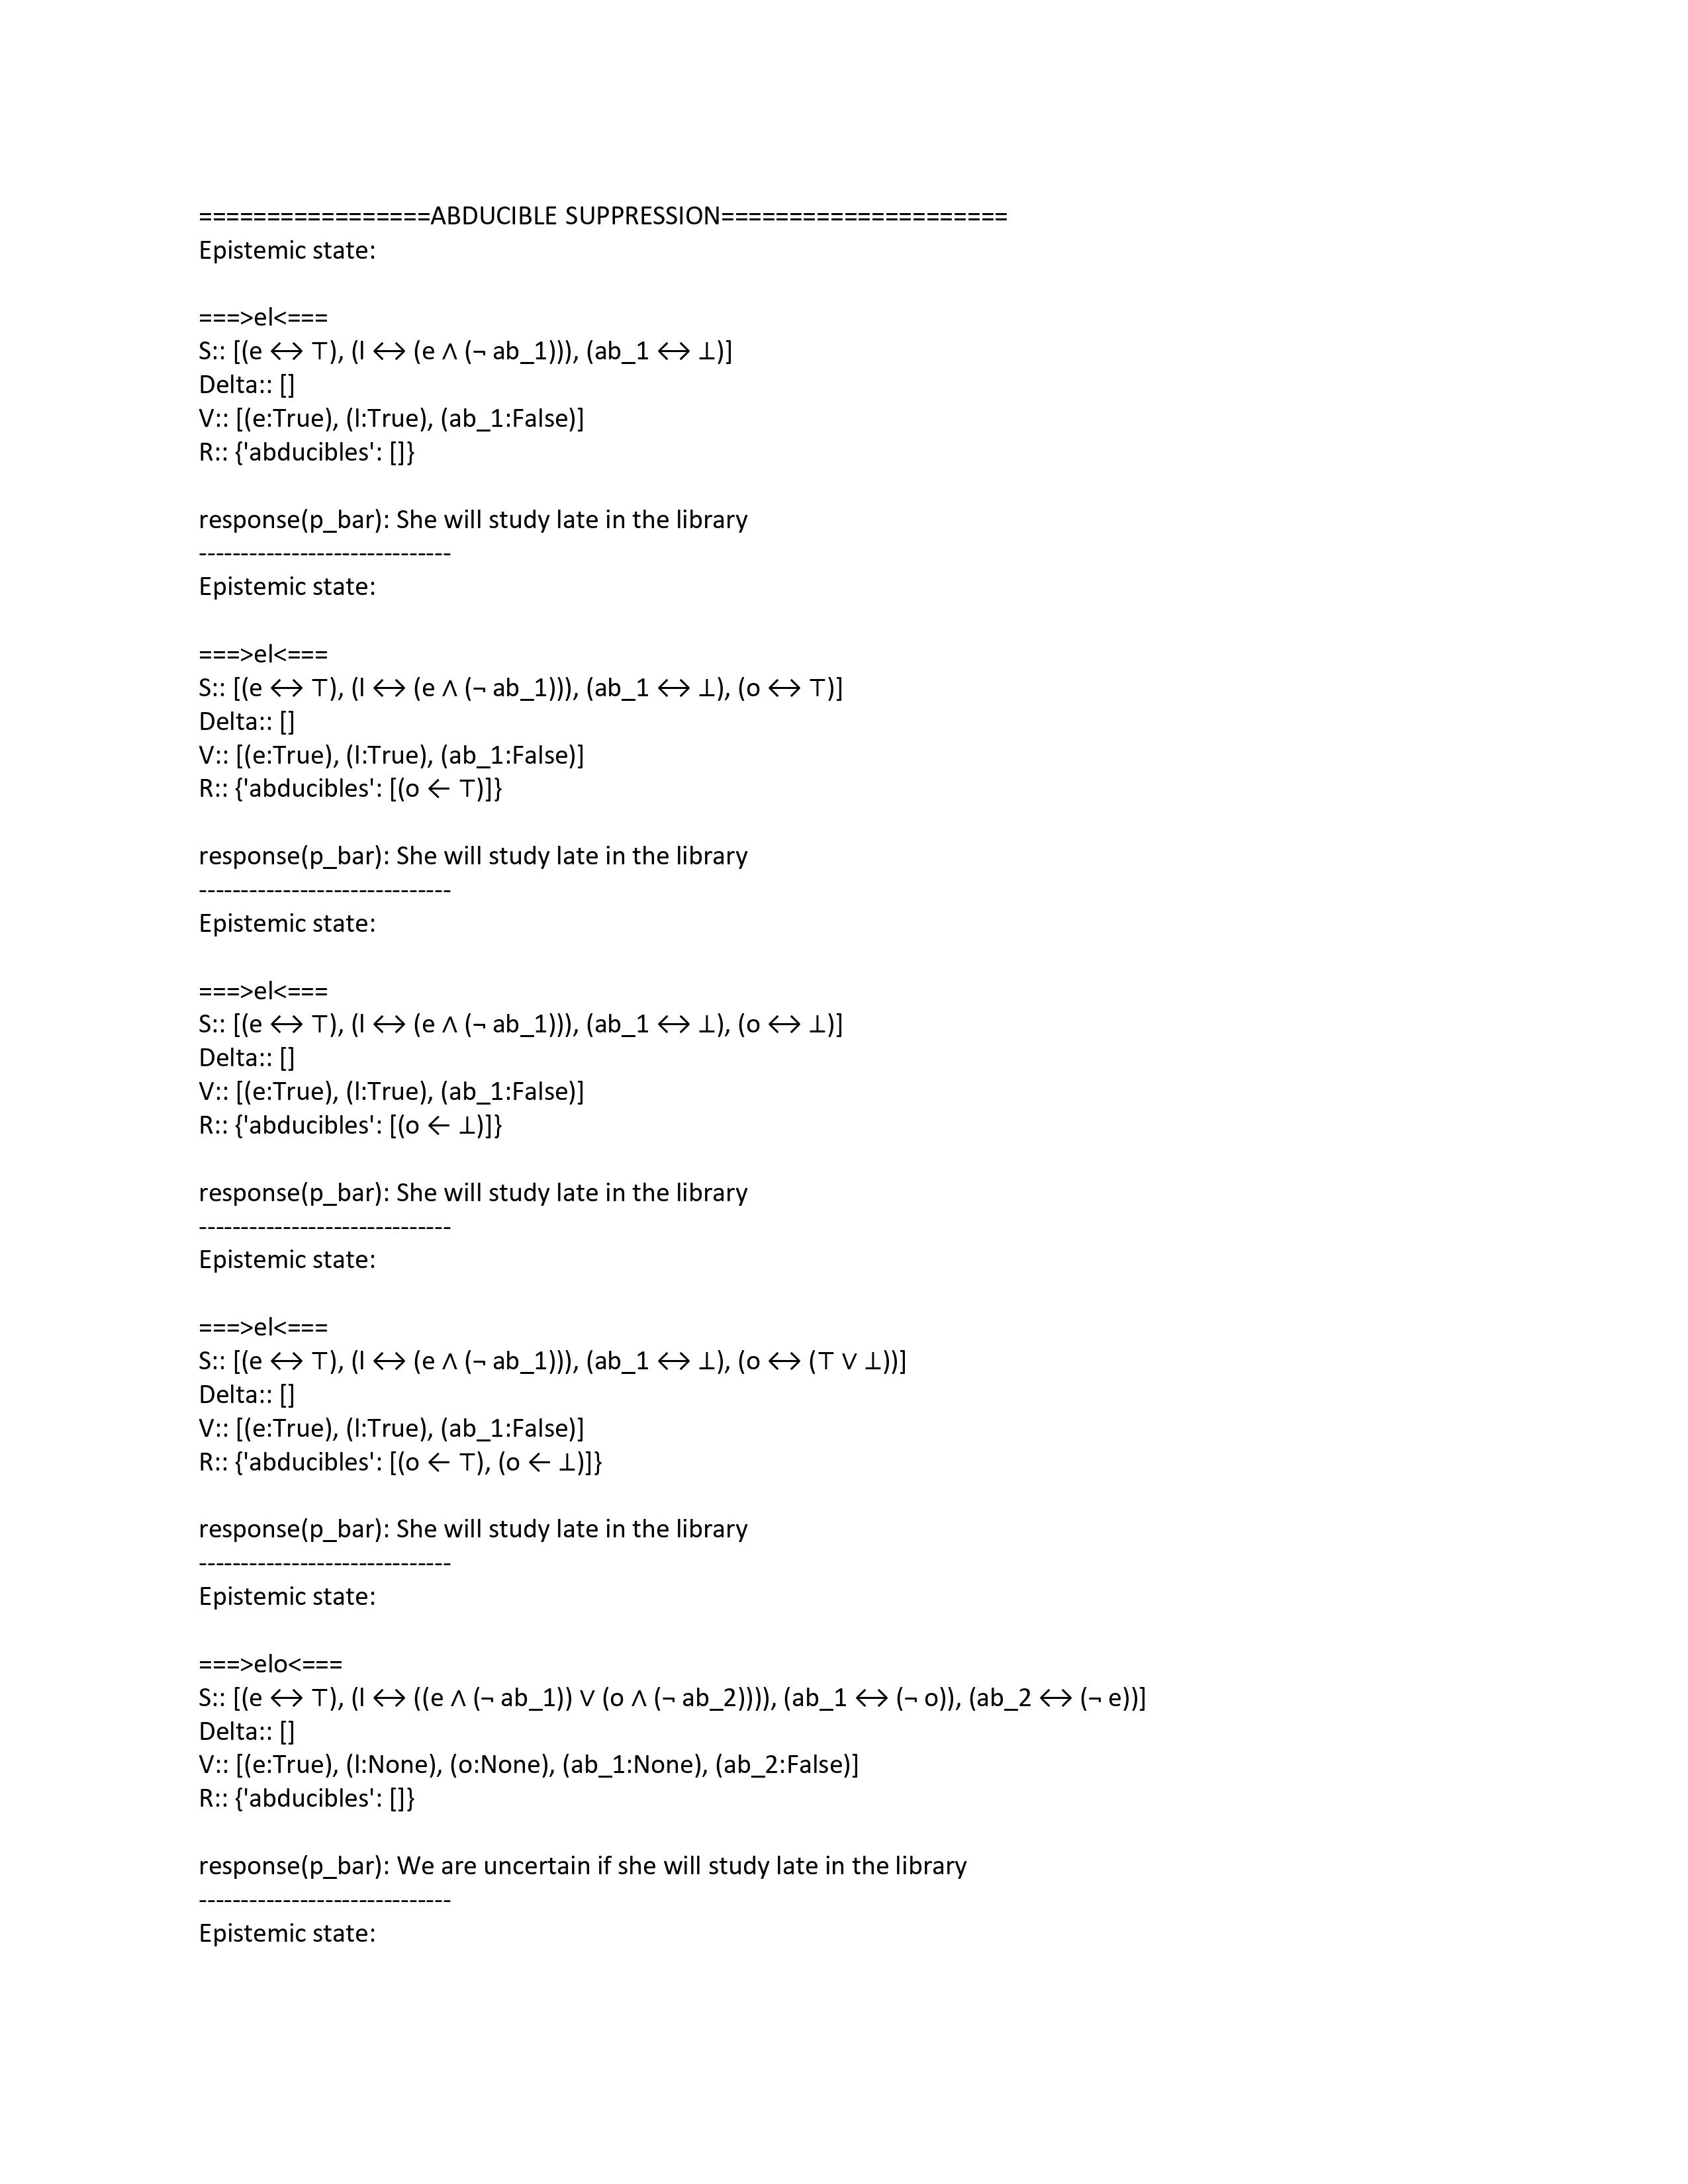
\includegraphics[width=\linewidth]{output1}
\caption{Epistemic states demonstrating that \texttt{addExp} can be used to model the individual case of the Suppression Task where Suppression is prevented. Shown for SCP $\mu=(\pi,f_\text{sup}())$, $\pi = (s_\text{dev} \longmapsto \texttt{addAB} \longmapsto \texttt{addExp} \longmapsto \texttt{wc} \longmapsto \texttt{semantic} )$. Part1.}
\label{fig:suppression_python}
\end{figure}
\begin{figure}
\centering 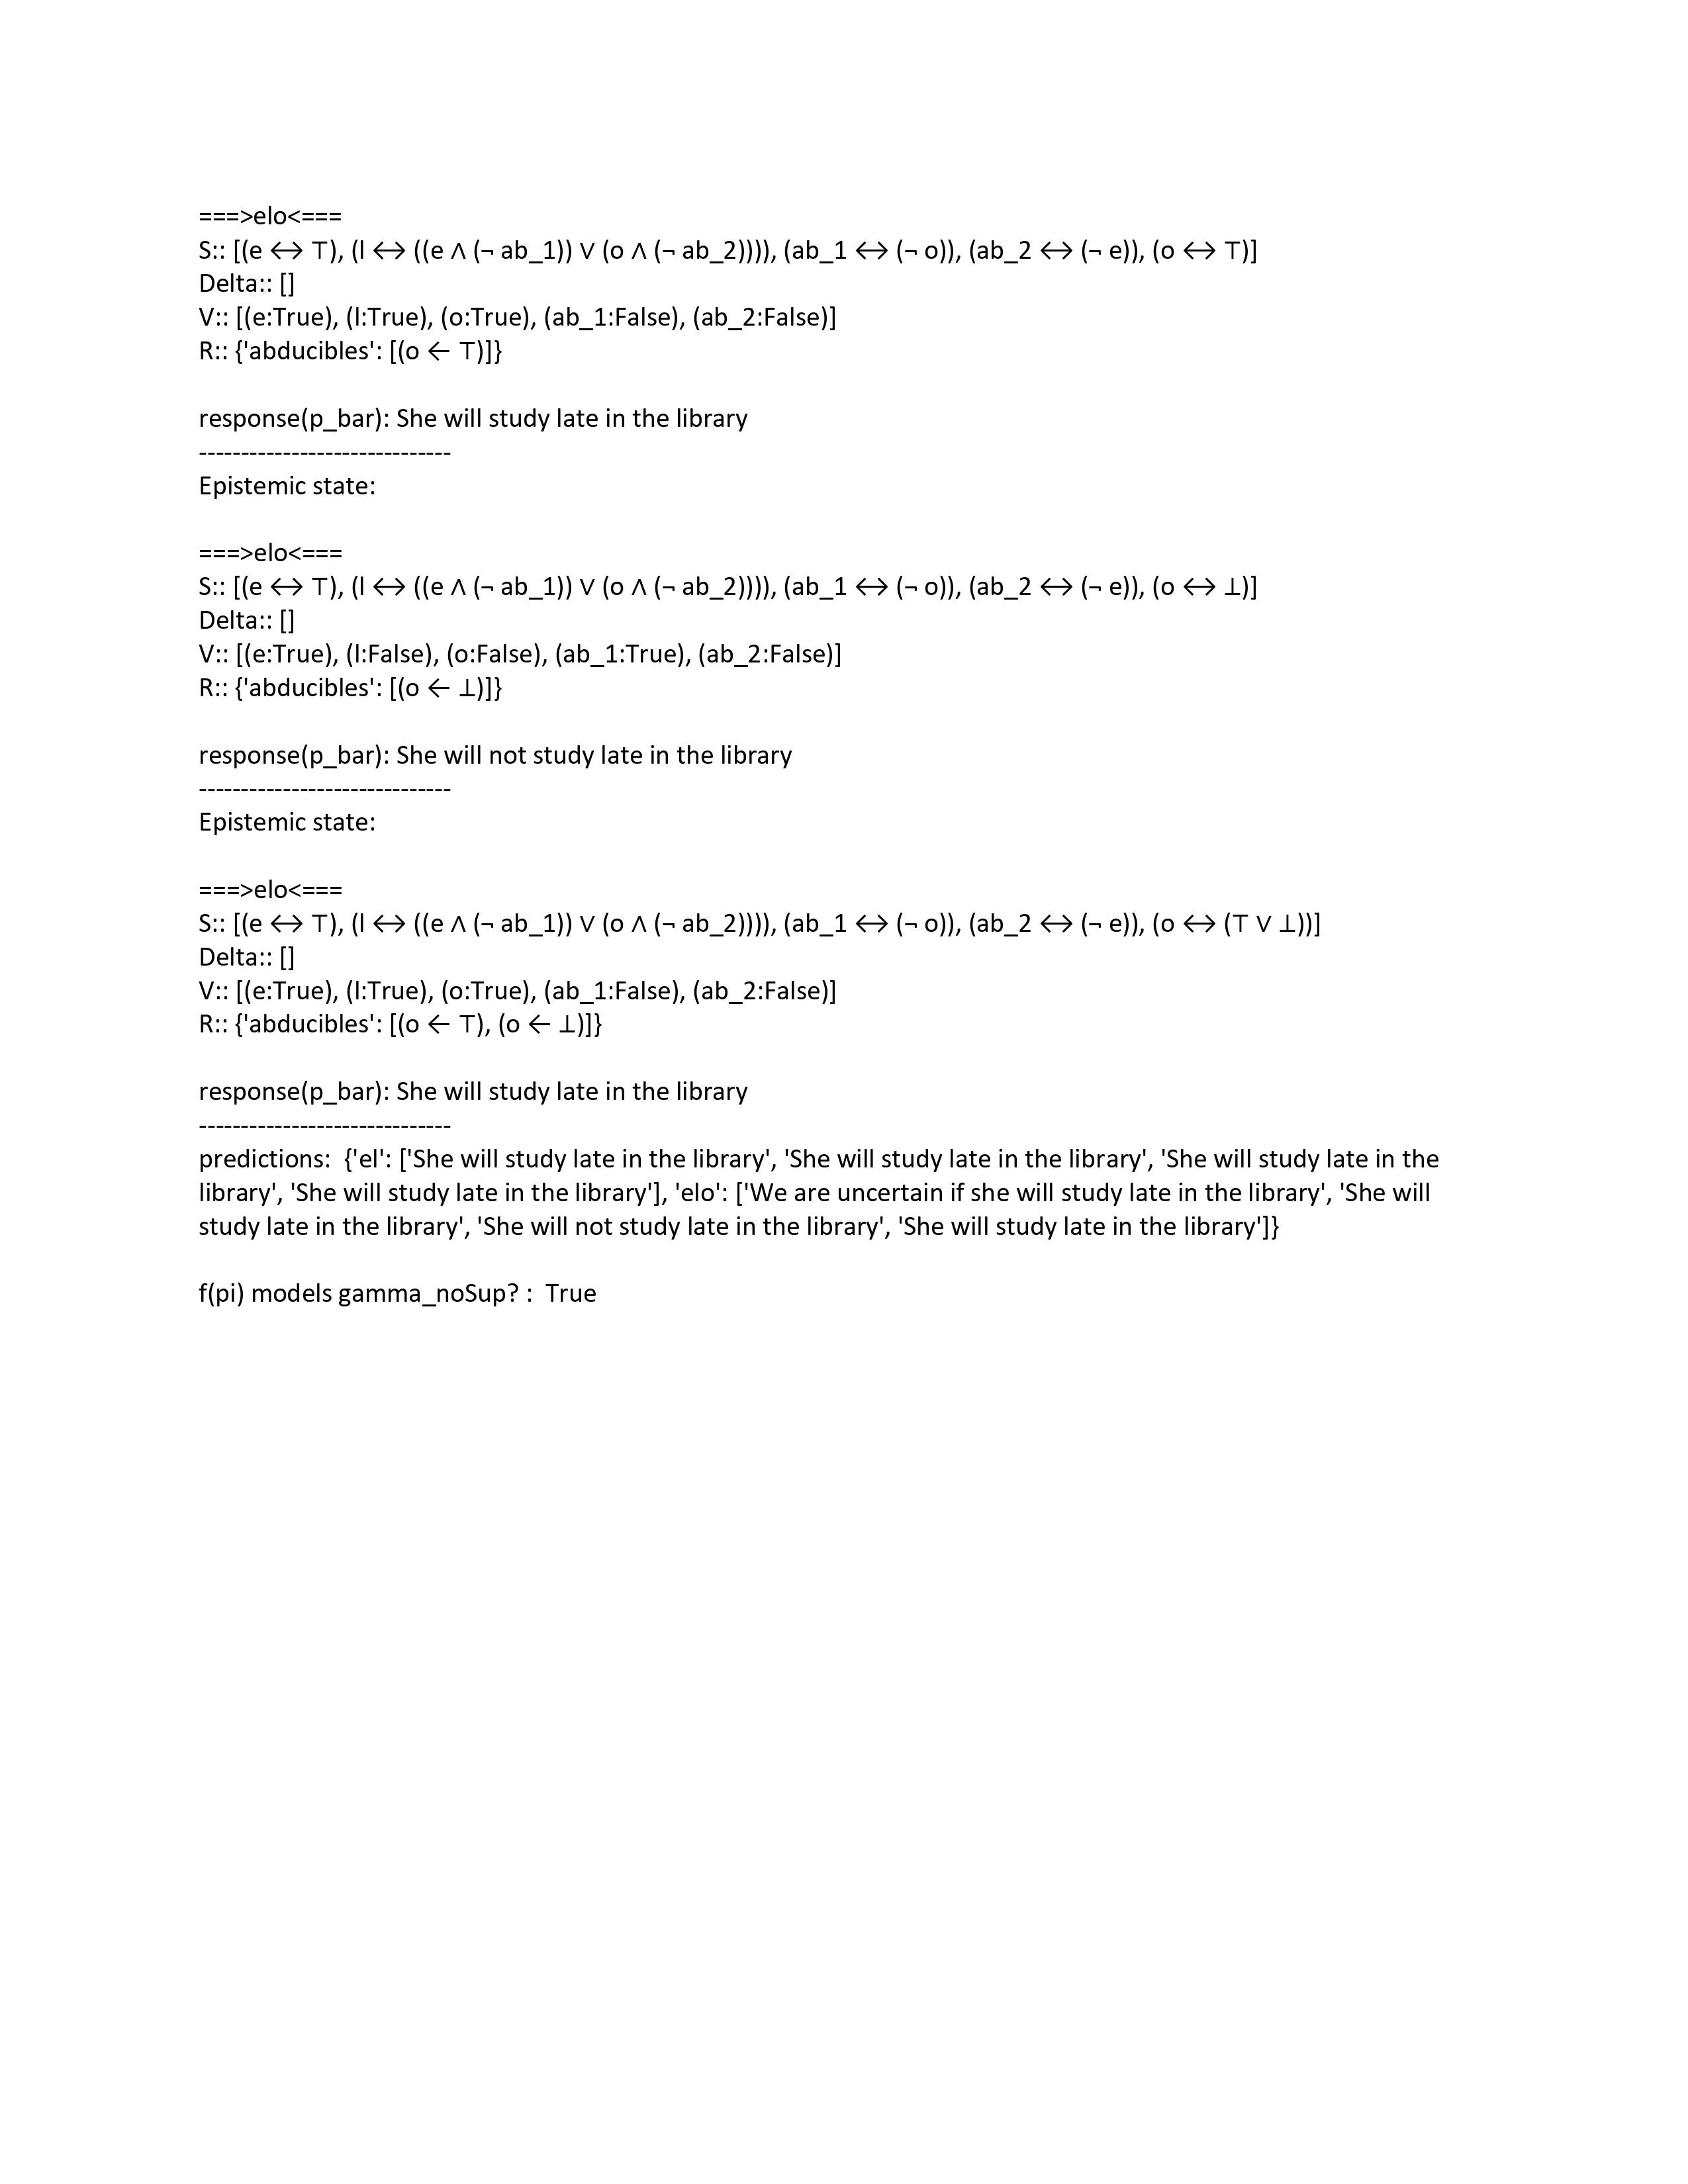
\includegraphics[width=\linewidth]{output2}
\caption{Epistemic states demonstrating that \texttt{addExp} can be used to model the individual case of the Suppression Task where Suppression is prevented. Shown for SCP $\mu=(\pi,f_\text{sup}())$, $\pi = (s_\text{dev} \longmapsto \texttt{addAB} \longmapsto \texttt{addExp} \longmapsto \texttt{wc} \longmapsto \texttt{semantic} )$. Part2.}
\label{fig:suppression_python2}
\end{figure}

\begin{figure}
\centering 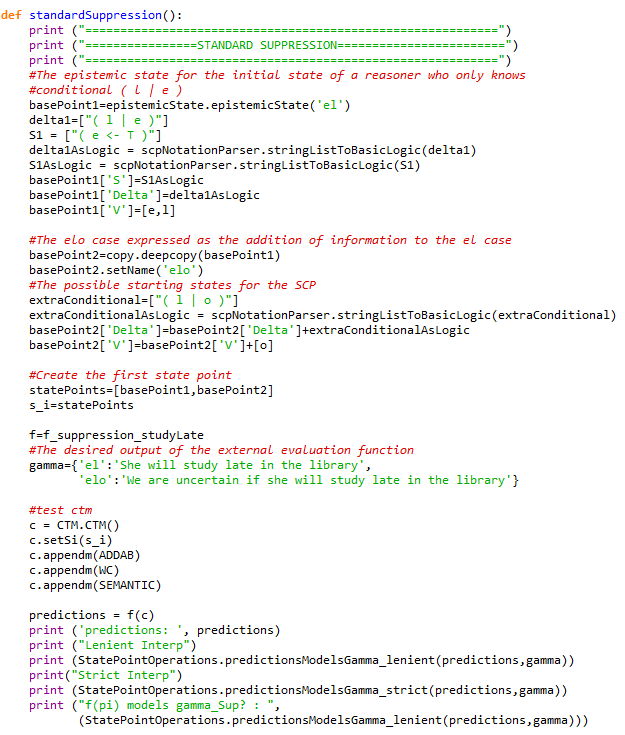
\includegraphics[width=\linewidth]{suppression_python}
\caption{Code snippet showing how the Suppression Task is modelled in the SCP Framework.}
\label{fig:sup_snippet}
\end{figure}

\FloatBarrier

\section*{Additional Tables}
\begin{table}[!htbp]
\begin{center}
\begin{tabular}{c | c c c c c c }
 & & $s_\text{WST}$ & \texttt{addAB} & \texttt{AddExp} & \texttt{wc} & \texttt{semantic}\\
\hline
 & 0 & -1 & -2 & -3 & -4 & -5\\
$s_\text{WST}$ & -1 & 3 & 2 & 1 & 0 & -1\\
\texttt{th} & -6 & -2 & 0.0 & -1.0 & -2.0 & -3.0
\end{tabular}
\caption{Extended Needleman-Wunsch comparison of $\mu_{D,3}$ to $\mu'_{D,7}$.}
\label{tbl:extal1}
\end{center}
\end{table}








\begin{table}[h!]
\begin{center}
\begin{tabular}{c | c c c c c c }
 & & $s_\text{WST}$ & \texttt{addAB} & \texttt{AddExp} & \texttt{wc} & \texttt{semantic}\\
\hline
 & 0 & -1 & -2 & -3 & -4 & -5\\
$s_\text{WST}$ & -1 & 3 & 2 & 1 & 0 & -1\\
\texttt{addAB} & -2 & 2 & 4 & 3 & 2 & 1\\
\texttt{addExp} & -3 & 1 & 3 & 5 & 4 & 3\\
\texttt{wc} & -4 & 0 & 2 & 4 & 6 & 5\\
\texttt{semantic} & -5 & -1 & 1 & 3 & 5 & 7
\end{tabular}
\caption{Extended Needleman-Wunsch comparison of $\mu_{D,3}$ to $\mu_{D,7}$.}
\label{tbl:extal2}
\end{center}
\end{table}
